\documentclass[t,12pt,numbers,fleqn]{beamer}
\usepackage{pgfpages} 
\usepackage{hyperref}
\usepackage{booktabs}

\hypersetup{colorlinks=true,
    linkcolor=blue,
    citecolor=blue,
    filecolor=blue,
    urlcolor=blue,
    unicode=false}
\urlstyle{same}

\mode<presentation>{}
 
%Information to be included in the title page:
\title{
    NavSafe\\
    \large A Safer Way To Get Around
}
\author{
    Arkin Modi\\
    Benson Hall\\
    Joy Xiao\\
    Leon So\\
    Timothy Choy
}
\institute{Department of Software and Computing, McMaster University}
\date{April 4, 2019}

\begin{document}
 
\frame{\titlepage}

%%%%%%%%%%%%%%%%%%%%%%%%%%%% Slide 2 %%%%%%%%%%%%%%%%%%%%%%%%%%%%%%%%%%%%%%%%%%%

\begin{frame}
\frametitle{NavSafe Objective}
NavSafe seeks to meet the following objective:
\begin{itemize}
    \item Determine the safest route for a person to travel on based on data of collisions in the Seattle area.
\end{itemize}
\end{frame}
 
%%%%%%%%%%%%%%%%%%%%%%%%%%%% Slide 3 %%%%%%%%%%%%%%%%%%%%%%%%%%%%%%%%%%%%%%%%%%%
\begin{frame}
\frametitle{Scope}
Features required to accomplish this project:
\begin{itemize}
    \item Searching algorithm
    \item Custom edge-weighted graph (bidirectional)
    \begin{itemize}
        \item[] Vertices = Intersection
        \item[] Edges = Path between pair of intersections
        \item[] Weight of an edge/vertex based on cumulative severity indices 
    \end{itemize}
    \item Shortest path algorithm (i.e., Dijkstra) to find safest route
\end{itemize}

\end{frame}
%%%%%%%%%%%%%%%%%%%%%%%%%%%% Slide 4 %%%%%%%%%%%%%%%%%%%%%%%%%%%%%%%%%%%%%%%%%%%
\begin{frame}
\frametitle{Motivation}
\begin{itemize}
    \item Vehicle collisions
    \begin{itemize}
        \item Potential risk of \textbf{injury} or \textbf{death}
    \end{itemize}
    \item Many high-risk intersections with flawed designs
    \begin{itemize}
        \item Factor out of the traveler’s control
        \item Mistakes by pedestrian or driver has a higher chance of being fatal in these intersections
    \end{itemize}
    \item Areas where flawed design could occur:
    \begin{itemize}
        \item Road width
        \item Speed limit
        \item Markings and signs
        \item Intersection infrastructure such as dividers and shoulders
    \end{itemize}
\end{itemize}
\end{frame}
%%%%%%%%%%%%%%%%%%%%%%%%%%% Slide 5 %%%%%%%%%%%%%%%%%%%%%%%%%%%%%%%%%%%%%%%%%%%%
\begin{frame}
\frametitle{Dataset(s) Used}
\begin{itemize}
    \item "Collisions" from Seattle GIS Open Data
    \begin{itemize}
        \item Number of Collisions
        \item Weather, road, and daylight conditions
        \item Type of collision (pedestrian/vehicle)
        \item Collision details (left/right turn, etc.)
        \item Severity of collision
    \end{itemize}
    \item Intersections dataset from the City of Seattle's data site
    \item Streets dataset from the City of Seattle's data site
\end{itemize}
\end{frame}
%%%%%%%%%%%%%%%%%%%%%%%%%%% Slide 6 %%%%%%%%%%%%%%%%%%%%%%%%%%%%%%%%%%%%%%%%%%%%
\begin{frame}
\frametitle{Requirements Specification}
\begin{itemize}
    \item Functional Requirements
    \begin{itemize}
        \item Read Module
        \item Collision ADT Module
        \item Intersection ADT Module
        \item Graphing Module
        %\item Sort Module   % dunno if we can include this
        \item Searching Module
    \end{itemize}
    \item[] % to create space
    \item Non-Functional Requirements
    \begin{itemize}
        \item Reliability
        \item Accuracy of Results
        \item Performance
        
        
%Performance issues:
%Went through many options for searching:
%Linear search (would work, but slow)
%Hashmaps (there would be two keys, which one to use?)
%-Factor in duplicate keys, using the same collision weighing 2-3 times, would skew results
%Symbol tables
%-Same problem as hashmaps
%2D array
%- Would need number index for each street
    %- Iterate through all collisions only once to do this
%- 2D array of some other data structure
    %- What data structure lol
    %- Potential problem of duplicates again?
%Key problems:
%- Duplicates
%- Indexing by both streets of an intersection
%- Don't know direction of a road


        \item Human-computer Interface Issues
        \item Constraints
        %perhaps bring up subjectiveness of our weighing?
    \end{itemize}
\end{itemize}
\end{frame}
%%%%%%%%%%%%%%%%%%%%%%%%%% Slide 7 %%%%%%%%%%%%%%%%%%%%%%%%%%%%%%%%%%%%%%%%%%%%%
\begin{frame}
\frametitle{Design Specification}
\begin{itemize}
    \item Read Module: Read CSV files and create ADTs to be used
    \item Graphing Module - Stage 1: Create custom edge-weighted graph
    \item Search Module: Search for collisions that occurred on an edge and factor them into the weighing of the edge
    \item Graphing Module - Stage 2: Using edge-weighted graph, find shortest path from starting intersection to destination intersection.
\end{itemize}
\end{frame}
%%%%%%%%%%%%%%%%%%%%%%%%%% Slide 8 %%%%%%%%%%%%%%%%%%%%%%%%%%%%%%%%%%%%%%%%%%%%%
\begin{frame}

% Verification and validation are independent procedures that are used together for checking that a product, service, or system meets requirements and specifications and that it fulfills its intended purpose. 

\frametitle{Verification and Validation}
Quality Control Procedures
\begin{itemize}
    \item Unit Testing
    \begin{itemize}
        \item Verify that individual units of code work as intended
    \end{itemize}
    %\item Continuous Integration Testing
    %\begin{itemize}
    %    \item Verify compatibility with existing modules
    %\end{itemize}
    \item System Testing
    \begin{itemize}
        \item Verify the program and specifications are aligned
    \end{itemize}
\end{itemize}
\end{frame}
%%%%%%%%%%%%%%%%%%%%%%%%%% Slide 9 %%%%%%%%%%%%%%%%%%%%%%%%%%%%%%%%%%%%%%%%%%%%%
\begin{frame}
\frametitle{Screenshot of implementation}
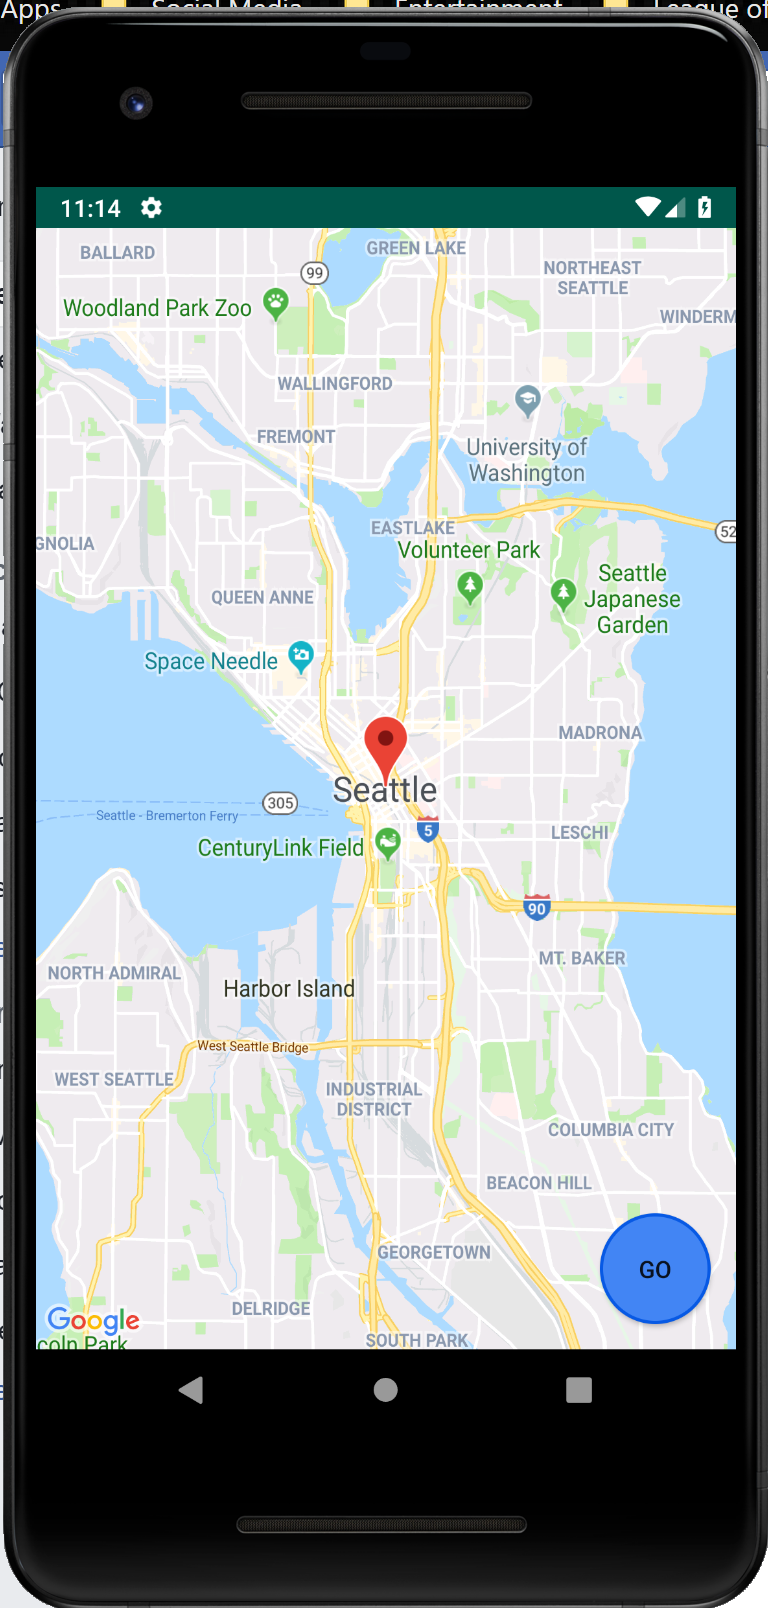
\includegraphics[scale=0.135]{screenshot.png}
\end{frame}

\end{document}